\documentclass[conference,a4paper]{IEEEtran}

% ============================================================
% COMP47360 Plug & Wifi ??IEEE Conference Report Template
%
% IMPORTANT:

% 1. Do not add geometry, titlesec, titling, setspace, or manual font-size changes: IEEEtran already controls the required layout.
% ============================================================

\usepackage[T1]{fontenc}
\usepackage{graphicx}
\usepackage{booktabs}
\usepackage{multirow}
\usepackage{amsmath,amssymb}
\usepackage{cite}
\usepackage{url}
\usepackage[hidelinks]{hyperref}
\usepackage{microtype}
\usepackage{balance}
\usepackage{xcolor}
\usepackage{tikz}
\usetikzlibrary{arrows.meta, positioning, fit}

% ---------- Draft switches ----------
\newif\ifincludecover
\includecovertrue       % Change to \includecoverfalse for standard IEEE output.

\newif\ifshowguidance
\showguidancetrue       % Change to \showguidancefalse before submission.

% Draft-only guidance. These boxes disappear when \showguidancefalse is used.
\newcommand{\guidance}[1]{%
  \ifshowguidance
    \par\smallskip
    \noindent\fcolorbox{gray}{gray!8}{%
      \parbox{\dimexpr\columnwidth-2\fboxsep-2\fboxrule\relax}{%
        \footnotesize\color{gray!75!black}\textbf{Draft guidance:} #1}}
    \par\smallskip
  \fi
}

% ---------- Paper metadata ----------
\title{Plug \& Wifi: An Integrated Platform for Discovering and Booking
Suitable Work and Study Venues}

\author{
\IEEEauthorblockN{Tzu Yu Chang, Youssef Bouarada, Sunmin Lee,\\
Wenfei Song, Peiyou Yao, and Adam Treanor}
\IEEEauthorblockA{
School of Computer Science, University College Dublin\\
Dublin, Ireland\\}
}

\begin{document}

% ============================================================
% OPTIONAL COURSE COVER PAGE ??not part of normal IEEE format
% ============================================================
\ifincludecover
\begin{titlepage}
  \centering
  \vspace*{2.2cm}

  {\Large\bfseries University College Dublin\par}
  \vspace{0.5cm}
  {\large School of Computer Science\par}

  \vfill

  {\LARGE\bfseries Plug \& Wifi\par}
  \vspace{0.4cm}
  {\Large Final Project Report\par}
  \vspace{0.8cm}
  {\large COMP47360 Research Practicum\par}

  \vfill

  \begin{tabular}{@{}ll@{}}
    \textbf{Team:} & Group 4 \\[0.35em]
    \textbf{Authors:} & Tzu Yu Chang \\
                      & Youssef Bouarada \\
                      & Sunmin Lee \\
                      & Wenfei Song \\
                      & Peiyou Yao \\
                      & Adam Treanor \\[0.35em]
    \textbf{Programme:} & MSc Computer Science (Conversion) \\
  \end{tabular}

  \vfill
  \ifshowguidance
    {\small\color{gray!75!black}
    Draft note: this optional module cover is not part of the standard
    IEEE conference-paper layout. Confirm whether it counts towards the
    module's page limit before submission.\par}
  \fi
\end{titlepage}
\setcounter{page}{1}
\fi

% ============================================================
% IEEE PAPER START
% ============================================================
\maketitle

\begin{abstract}
\guidance{Target: approximately 150--200 words (about 0.25--0.30 page).
State the problem and objective, the integrated methodology, the principal
quantitative or evaluative results, and the main contribution or innovation.
Avoid citations and undefined abbreviations.}
\textit{[Insert the final abstract here.]}
\end{abstract}

\begin{IEEEkeywords}
venue discovery, workspace recommendation, busyness prediction,
location-based services, booking systems, conversational search
\end{IEEEkeywords}

% ============================================================
% I. INTRODUCTION ??target: 0.60--0.70 page
% Rubric weight: 10%
% Owner: Youssef
% ============================================================
\section{Introduction}
\label{sec:introduction}
\guidance{Target: 0.60--0.70 page. Establish the motivation and context,
define the user problem, identify the gap, state the project objectives and
research or engineering questions, summarise the contribution, and end with
a brief paper roadmap.}

\subsection{Background and Motivation}
\textit{[Introduce the difficulty of finding suitable, available venues for
work or study.]}

\subsection{Problem Definition and Objectives}
\textit{[Define the problem, target users, project scope, objectives, and
principal contributions.]}

% ============================================================
% II. LITERATURE REVIEW ??target: 1.20--1.30 pages
% Rubric weight: 15%
% Owner: Youssef
% ============================================================
\section{Literature Review}
\label{sec:literature-review}
\guidance{Target: 1.20--1.30 pages. Critically compare relevant scientific
literature and similar platforms. Cover location-based venue discovery,
context-aware or multi-criteria recommendation, busyness estimation,
booking systems, and conversational search. Conclude by identifying the
specific gap addressed by Plug \& Wifi.}

\subsection{Venue Discovery and Similar Platforms}
\textit{[Compare relevant commercial systems and research prototypes.]}

\subsection{Context-Aware Recommendation and Busyness Prediction}
\textit{[Synthesise research methods, evidence, limitations, and relevance.]}

\subsection{Research Gap}
\textit{[Explain how the reviewed work motivates the integrated design of
Plug \& Wifi.]}

% ============================================================
% III. METHODOLOGY ??target: 2.10--2.30 pages
% Rubric weight: 20%
% Owners: Alex, Sunmin, Peiyou, Wenfei
% ============================================================
\section{Methodology}
\label{sec:methodology}
\guidance{Target: 2.10--2.30 pages in total. For each major decision use:
requirement or problem, selected approach, implementation, justification,
and trade-off. Include a compact architecture figure and avoid turning the
section into a feature list.}

\subsection{Project Management, Integration and Deployment}
\label{sec:project-management}

We managed development through an Agile, iterative process in which the
backlog and sprint objectives were continuously revised according to
delivery progress, technical feasibility, cross-component dependencies,
and the remaining project capacity. Jira was selected over Google Sheets
because its epics, stories, tasks, ownership fields, workflow states,
burndown charts, and timeline views provided stronger traceability and
progress control. Sprint planning, progress reviews, integration meetings,
and Jira status monitoring enabled us to identify blockers and redistribute
or redefine incomplete work rather than treating the initial backlog as a
fixed specification. During the final sprint, we deliberately converged
the scope around complete, demonstrable user journeys. Third-party payment
integration, QR-code check-in, floor plans, booking extensions,
booking-history personalisation, and external venue photographs were
deferred so that the core search, availability, booking, recommendation,
chatbot, provider, and administration workflows could be integrated and
prepared for the final demonstration.

Repository integration was controlled through a documented branch and
pull-request workflow. The monorepo contained the Web, Mobile, Backend, and
Data/ML components, allowing shared API contracts and cross-component
changes to be validated within one integration baseline. The
\texttt{main} branch represented production-ready code, while
\texttt{develop} was used for continuous integration. Development was
isolated in Jira-linked feature branches, and direct commits to either
protected branch were prohibited. Before opening a pull request,
contributors synchronised with the latest \texttt{develop} branch and
rebased their work to expose conflicts before integration. Pull requests
were merged only after build, lint, and test checks succeeded, conflicts
and API compatibility were reviewed, and at least one peer approval was
obtained. Squash or linear-history merging was used to keep revisions
traceable and reduce integration ambiguity.

Deployment was implemented as a containerised CI/CD workflow rather than
through manually maintained application servers. Docker encapsulated the
application runtime and dependencies, producing reproducible artefacts
across local, CI, and production environments. Cloud Build triggers were
aligned with the branch workflow and executed YAML-defined stages to build
the relevant Docker image, publish it to Artifact Registry, and deploy a
new revision to Cloud Run. GCP was selected because of the available
USD~300 credit and its integration with Google Maps APIs, Cloud Storage,
and the wider application environment. Compared with maintaining dedicated
AWS EC2 instances, Cloud Run reduced infrastructure administration and
allowed services to scale down during inactivity. We managed the resulting
cold-start trade-off by retaining a minimum instance for critical services.
Cloud Run revisions, application logs, health and diagnostic endpoints,
environment variables, and production-database connectivity checks were
used to diagnose failed builds and HTTP 500/502 responses and to validate
new deployments. This combination of repository guardrails,
containerisation, automated deployment, and runtime monitoring allowed the
integrated product to remain continuously deployable throughout
development.

\begin{figure}[!htbp]
\centering
\resizebox{\columnwidth}{!}{%
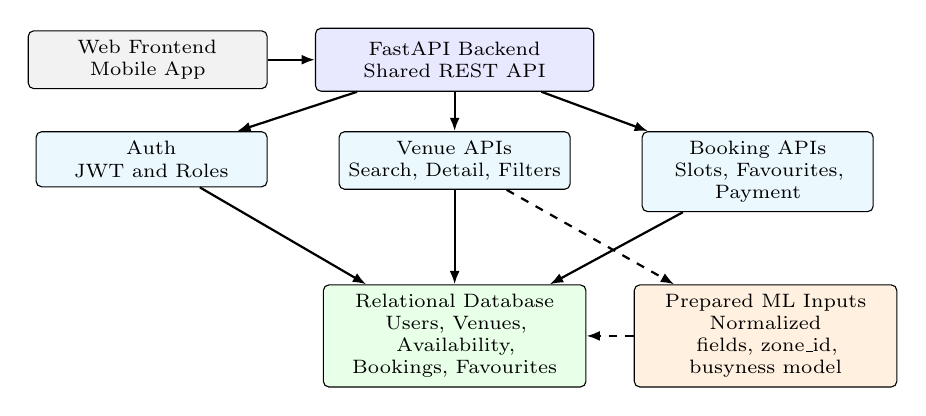
\begin{tikzpicture}[
    font=\scriptsize,
    node distance=5mm and 6mm,
    client/.style={draw, rounded corners=2pt, align=center, minimum height=7mm, text width=28mm, fill=gray!10},
    core/.style={draw, rounded corners=2pt, align=center, minimum height=8mm, text width=33mm, fill=blue!9},
    api/.style={draw, rounded corners=2pt, align=center, minimum height=7mm, text width=27mm, fill=cyan!8},
    data/.style={draw, rounded corners=2pt, align=center, minimum height=8mm, text width=31mm, fill=green!9},
    ml/.style={draw, rounded corners=2pt, align=center, minimum height=8mm, text width=31mm, fill=orange!12},
    arrow/.style={-{Latex[length=1.7mm]}, thick},
    dashedarrow/.style={-{Latex[length=1.7mm]}, thick, dashed}
]

\node[client] (clients) {Web Frontend\\Mobile App};
\node[core, right=of clients] (backend) {FastAPI Backend\\Shared REST API};

\node[api, below left=of backend] (auth) {Auth\\JWT and Roles};
\node[api, below=of backend] (venueapi) {Venue APIs\\Search, Detail, Filters};
\node[api, below right=of backend] (bookingapi) {Booking APIs\\Slots, Favourites, Payment};

\node[data, below=12mm of venueapi] (db) {Relational Database\\Users, Venues, Availability,\\Bookings, Favourites};
\node[ml, right=of db] (mlartifacts) {Prepared ML Inputs\\Normalized fields, zone\_id,\\busyness model};

\draw[arrow] (clients) -- (backend);
\draw[arrow] (backend) -- (auth);
\draw[arrow] (backend) -- (venueapi);
\draw[arrow] (backend) -- (bookingapi);

\draw[arrow] (auth) -- (db);
\draw[arrow] (venueapi) -- (db);
\draw[arrow] (bookingapi) -- (db);
\draw[dashedarrow] (venueapi) -- (mlartifacts);
\draw[dashedarrow] (mlartifacts) -- (db);


\end{tikzpicture}%
}
\caption{Backend architecture and shared data flow for Plug \& Wifi.}
\label{fig:backend_architecture}
\end{figure}
\subsection{System Architecture, Backend and Database}
The system was designed around a backend-centred REST architecture. Instead of placing search, booking, authentication, and recommendation logic separately in the web and mobile clients, both clients communicate with the same FastAPI backend through a shared REST API. This approach was chosen because the web and mobile applications needed to receive the same venue data, apply the same business rules, and remain consistent as features evolved. REST's client-server and uniform-interface constraints support this separation of concerns and allow clients and servers to evolve independently \cite{fielding2000rest}. FastAPI was selected because its typed Python development model and automatic OpenAPI documentation helped the team test endpoints and align API contracts during implementation \cite{fastapi_docs}.

The database design followed the same principle of separating internal data structure from client response format. The backend does not store venue data as one frontend-shaped record. Instead, it models the main business entities separately, including venues, availability slots, bookings, favourites, and reviews, and then assembles them into consistent API responses for venue list, venue detail, availability, booking, and favourite flows. This reduced duplicated data and helped preserve consistency across shared records \cite{codd1970relational}. It also matched the purpose of OpenAPI-style interface descriptions, where clients can consume a clearly defined API without guessing how server-side data is organised \cite{openapi_spec}.

Authentication and access control are handled on the backend using JWT bearer tokens. When a protected request is received, the backend validates the token, identifies the current user, and then applies the relevant user or role-based checks. This is especially important for booking creation. The booking API does not trust a \texttt{user\_id} sent from the frontend; instead, the booking owner is assigned from the authenticated user resolved by the backend. This prevents a user from creating a booking under another account by modifying the request payload. The same principle is used for user-specific operations such as creating or removing favourite venues.

The venue discovery API was extended to support the product flows required by the frontend and mobile app. The venue list endpoint returns pagination metadata such as \texttt{total\_items}, \texttt{total\_pages}, and \texttt{has\_more}, which allows the frontend to display multiple page buttons instead of treating each response as an isolated page. The same endpoint also supports advanced filters including Wi-Fi availability, plug access, venue type, accessibility, certification fields, location radius, and selected date or time. Public discovery queries consistently exclude venues that are suspended or still pending administrator approval, so newly submitted provider records are hidden until they are approved.

Several backend endpoints were added to replace incomplete or mock-based flows with real API-supported behaviour. The availability endpoint returns bookable time slots for a selected venue, including the date, start time, end time, availability status, and remaining seats. Booking creation keeps the existing validation for venue existence, available slots, overlapping bookings, and seat capacity. A mock payment confirmation endpoint was also added for demonstration purposes: a booking first enters a pending payment state, and the payment confirmation step then updates it to paid, failed, or unchanged depending on the demo card result. This gives the frontend and mobile app a realistic checkout flow without integrating a third-party payment provider.

The backend response contract was aligned so that web and mobile clients can consume the same field names and data types. For example, venue responses expose canonical fields such as \texttt{hourly\_price}, \texttt{plug\_access}, \texttt{lat}, \texttt{lon}, \texttt{seat\_capacity}, \texttt{amenity\_tags}, and \texttt{rules\_text}. Boolean filter fields are returned as true or false values with safe defaults, reducing the need for frontend-side inference or duplicated mapping logic. Deprecated noise-related fields were removed from active API responses and application logic to avoid conflicting data contracts.

Recommendation-related values are also calculated or attached through the backend so that clients receive consistent venue ranking information. The ML pipeline prepares reusable venue features such as normalized Wi-Fi, plug, rating, bus, train, and zone values. The backend then applies these features during real API requests. Suitability score is calculated as a deterministic 0--100 value and can be used for recommended sorting after filters have already been applied. Area busyness is handled separately from venue availability: the backend loads the zone-based busyness model once, predicts surrounding-area busyness for the selected date and time, reuses predictions for venues in the same zone, and returns \texttt{busyness\_score}, \texttt{busyness\_label}, and \texttt{busyness\_predicted\_for}. This design keeps security-sensitive and shared business logic on the backend, while giving the web and mobile clients a stable API contract for venue discovery and booking.

\subsection{Web and Mobile Applications}
\textit{[Explain the shared API contract and the design of search,
autocomplete, Map/List interaction, filters, booking, favourites, provider
and administrator flows, and mobile route planning.]}

\subsection{Recommendation and Conversational Search}
\textit{[Explain the Suitability Score, preference handling, database-grounded
chatbot behaviour, structured filters, fallback behaviour, and safeguards
against recommending non-existent venues.]}

% ============================================================
% IV. DATA ANALYTICS AND VISUALIZATION ??target: 1.00--1.10 pages
% Rubric weight: 15%
% Owner: Adam
% ============================================================
\section{Data Analytics and Visualization}
\label{sec:data-analytics}
\guidance{Target: 1.00--1.10 pages. Report the source and properties of the
data, cleaning and preprocessing, feature engineering, train/test strategy,
model selection and rationale, and how outputs are visualised in the
product. Include concise, interpretable quantitative graphics rather than
decorative screenshots.}

\subsection{Data Collection and Preprocessing}
\textit{[Describe sources, missing data, transformations, zone mapping,
temporal variables, and data-quality limitations.]}

\subsection{Feature Engineering and Model Selection}
\textit{[Explain features, candidate methods, final model, hyperparameters,
and selection rationale.]}

\subsection{Product-Level Visualization}
\textit{[Explain how Busyness Score, labels, Suitability Score, map markers,
and other analytical outputs are communicated to users.]}

% ============================================================
% V. EVALUATION AND RESULTS ??target: 1.40--1.60 pages
% Rubric weight: 20%
% Owner: Alex coordinates; all members provide evidence
% ============================================================
\section{Evaluation and Results}
\label{sec:evaluation}
\guidance{Target: 1.40--1.60 pages. Report methods and measurable results,
not only completed features. Include unit/component and end-to-end testing,
ML train/test results, UI/user evaluation and feedback, design-decision
evidence, deployment observations, and limitations. A compact results table
can use space more efficiently than multiple screenshots.}

\subsection{Software and Integration Testing}

As the first layer of quality assurance, every pull request targeting
\texttt{develop} was evaluated by a full-stack GitHub Actions workflow before
being eligible for merge. The workflow created a consistent Ubuntu-based test
environment and validated both application layers. For the Python backend,
Ruff performed static syntax and defect checks, followed by the complete
Pytest suite. For the React frontend, dependencies were installed using
\texttt{npm ci} and a production Vite build was executed. The workflow was
also rerun after changes were merged into \texttt{develop}, providing an
additional check of the integrated branch.



The CI gate successfully detected defects that could otherwise have entered
the shared integration branch. In one backend pull request, Ruff reported 15
syntax errors in \texttt{main.py}. Inspection showed that unresolved Git
conflict markers, including \texttt{<<<<<<<}, \texttt{=======}, and
\texttt{>>>>>>>}, had remained in the source file. The failed check prevented
the pull request from being merged until the conflict was resolved. In a
second case, all 100 backend tests passed, but the frontend production build
failed after transforming 2,186 modules. Vite traced the failure to mismatched
JSX structure in \texttt{HomePage.tsx}, where a \texttt{div} element lacked a
corresponding closing tag. After the JSX structure was corrected, the pipeline
was rerun successfully.



In the latest recorded successful run, Ruff reported no errors, all 148
backend tests passed in 60.89 seconds, and the frontend production bundle was
built successfully in 1.19 seconds. These results demonstrate that the CI
workflow operated as an effective pre-merge quality gate across backend
syntax, automated tests, and frontend build integrity.

\subsection{Machine-Learning Evaluation}
\textit{[Report the train/test split, baselines, metrics, numerical results,
interpretation, error analysis, and threats to validity.]}

\subsection{User-Interface Evaluation}
\textit{[Report participants, tasks, procedure, task-completion rate, time or
error measures, rating scales, qualitative feedback, and resulting changes.]}

\subsection{Deployment and Runtime Results}
\label{sec:deployment-results}

Merges into the \texttt{develop} branch automatically triggered separate Cloud
Build pipelines for the frontend and backend. Each pipeline built the
component-specific Docker image, pushed it to Artifact Registry, and deployed a
new Cloud Run revision. Containerisation ensured consistent dependencies and
runtime configurations between development and production.

On 24 July 2026, both services were successfully deployed from commit
\texttt{107cc80}. The frontend deployment completed in 84.23 seconds, while the
backend pipeline, including validation, completed in 164.75 seconds. The backend
smoke test returned HTTP~200 and confirmed successful PostgreSQL connectivity.
The database was hosted on Cloud SQL with 2~vCPUs and 8~GB of memory.

The backend Cloud Run service used 1~vCPU and 2~GiB of memory, while the frontend
used 1~vCPU and 256~MiB. Both services supported 80 concurrent requests per
instance, a 300-second request timeout, and a maximum of five instances.

Runtime monitoring identified a backend cold-start issue. Before adjustment,
requests to \texttt{/api/venues} took 7.647 and 1.738 seconds. After changing the
backend minimum-instance setting from zero to one, a subsequent request returned
HTTP~200 in 145 milliseconds. No recurrence of the original scale-from-zero
behaviour was observed during later checks.

Median request latency generally remained below one second, although occasional
multi-second P95 and P99 peaks were recorded. As production traffic was limited,
these results demonstrate deployment stability and the effectiveness of the
cold-start mitigation, but not large-scale system capacity. Controlled load
testing therefore remains future work.

% ============================================================
% VI. CONCLUSION AND FUTURE WORK ??target: 0.60--0.70 page
% Rubric weight: 10%
% Owner: Alex
% ============================================================
\section{Conclusion and Future Work}
\label{sec:conclusion}
\guidance{Target: 0.60--0.70 page. Answer the project objectives using the
reported results, state the contribution, acknowledge technical and
evaluation limitations, and propose realistic future work with its expected
impact. Do not introduce new evidence here.}


This project delivered a fully deployed platform that supports venue discovery, decision-making, and booking. A key contribution was the integration of a machine-learning-based Busyness Score and an AI-powered chatbot with real venue and availability data. Together with the Suitability Score, these features transformed the available data into practical information that helps users compare venues and make more informed decisions. The successful cloud deployment and end-to-end integration also demonstrated the feasibility of the proposed system beyond a standalone prototype.

However, the current system is limited to venues in Manhattan and operates on a relatively small dataset. Its recommendation features do not yet incorporate long-term user behaviour or booking history, while payment, identity verification, and administrative processes remain simplified. Future development should therefore prioritise secure third-party payment integration and QR-code-based arrival verification. Expanding the platform to additional regions and larger datasets, followed by controlled load and performance testing, would also be necessary to evaluate its scalability and support wider real-world adoption.



% ============================================================
% REFERENCES ??rubric weight: 5%
% Confirm whether references count towards the module page limit.
% Use IEEE numbered citations in order of first appearance.
% ============================================================
\balance
\begin{thebibliography}{00}

\bibitem{fielding2000rest}
R. T. Fielding, ``Architectural Styles and the Design of Network-based Software Architectures,'' Ph.D. dissertation, University of California, Irvine, 2000. [Online]. Available: https://ics.uci.edu/~fielding/pubs/dissertation/rest\_arch\_style.htm

\bibitem{fastapi_docs}
FastAPI, ``OpenAPI docs,'' FastAPI Documentation. [Online]. Available: https://fastapi.tiangolo.com/reference/openapi/docs/

\bibitem{codd1970relational}
E. F. Codd, ``A relational model of data for large shared data banks,'' \textit{Communications of the ACM}, vol.~13, no.~6, pp.~377--387, 1970.

\bibitem{openapi_spec}
OpenAPI Initiative, ``OpenAPI Specification v3.1.1,'' 2024. [Online]. Available: https://spec.openapis.org/oas/v3.1.1.html

\end{thebibliography}

\end{document}
